\documentclass[conference]{IEEEtran}

\usepackage{amsmath}
\usepackage{amssymb}
\usepackage{blindtext}
\usepackage{booktabs}
\usepackage{caption}
\usepackage{graphicx}
\usepackage[utf8]{inputenc}
\usepackage{multirow}
\usepackage[group-separator={,}]{siunitx}
\usepackage[x11names, rgb, dvipsnames]{xcolor}
\usepackage{xfrac}
\usepackage[perpage]{footmisc}
\usepackage[hidelinks=true]{hyperref}

\usepackage{tikz}
\usetikzlibrary{shapes}

\bibliographystyle{alpha}

\DeclareMathOperator{\orig}{orig}
\DeclareMathOperator{\dest}{dest}

\DeclareMathOperator{\calls}{calls}
\DeclareMathOperator{\etime}{time}
\DeclareMathOperator{\sms}{sms}
\DeclareMathOperator{\contacts}{contacts}

\DeclareMathOperator{\incalls}{incalls}
\DeclareMathOperator{\intime}{intime}
\DeclareMathOperator{\insms}{insms}
\DeclareMathOperator{\incontacts}{incontacts}

\DeclareMathOperator{\outcalls}{outcalls}
\DeclareMathOperator{\outtime}{outtime}
\DeclareMathOperator{\outsms}{outsms}
\DeclareMathOperator{\outcontacts}{outcontacts}

\DeclareMathOperator{\inner}{inner}
% \DeclareMathOperator{\outer}{outer}

\newcommand{\todo}[1]{\textbf{\color{red} TODO:\@ #1}}
\newcommand{\maybe}[1]{\footnote{\color{red} #1}}

\newcommand{\NA}{---}
\newcommand{\ct}[1]{\multicolumn{1}{c}{#1}}

\DeclareMathOperator{\ego}{Ego}
\DeclareMathOperator{\cat}{Cat}

\DeclareMathOperator{\train}{train}
\DeclareMathOperator{\test}{test}

\newcommand{\noimage}{%
  \setlength{\fboxsep}{-\fboxrule}
  \fbox{\phantom{\rule{\columnwidth}{100pt}}}
}
\newcommand{\includegraphicsmaybe}[1]{\IfFileExists{#1}{\includegraphics[width=\columnwidth]{#1}}{\noimage}}

\renewcommand{\thefootnote}{\fnsymbol{footnote}}
\captionsetup[table]{skip = 2ex}

\title{Comparison of Feature Extraction Methods and Predictors for Income Inference}

\author{%
\IEEEauthorblockN{%
	Martin Fixman\IEEEauthorrefmark{1},
	Carlos Sarraute\IEEEauthorrefmark{2},
	Many Others\IEEEauthorrefmark{2}
}
\IEEEauthorblockA{\IEEEauthorrefmark{1}Universidad de Buenos Aires, Argentina}
\IEEEauthorblockA{\IEEEauthorrefmark{2}Grandata Labs, Bartolomé Cruz 1818, Vicente López, Buenos Aires, Argentina}
\IEEEauthorblockA{martinfixman@gmail.com, charles@grandata.com}
}

\begin{document}
\maketitle

\begin{abstract}
%The explosion of mobile phone communications in the last years occurs at a moment where data processing power increases exponentially.  Thanks to those two changes in a global scale, the road has been opened to use mobile phone communications to generate inferences and characterizations of mobile phone users.
%In this work, we use the communications network, enriched by a set of users' attributes, to gain a better understanding of the demographic features of a population. Namely, we use
%call detail records and banking information to infer the income of each person in the graph.

%\todo{We need to rewrite the abstract.}

In this work, we examine the socio-economic correlations present among users in a mobile phone network in Mexico. First, we find that the distribution of income for a subset of users --for which we have income information given by a large bank in Mexico-- follows closely, but not exactly, the income distribution for the whole population of Mexico. We also show the existence of a strong socio-economic homophily in the mobile phone network, where users linked in the network are more likely to have similar income. The main contribution of this work is that we leverage this homophily in order to propose a methodology, based on Bayesian statistics, to infer the socio-economic status for a large subset of users in the network (for which we have no banking information). With our proposed algorithm, we achieve an accuracy of 0.71 in a two-class classification problem (low and high income) which significantly outperforms a simpler method based on a frequentist approach. Finally, we extend the two-class classification problem to multiple classes by using the Dirichlet distribution.

\end{abstract}

% !TEX root = tesis.tex

\chapter{Introduction}

% MOTIVATION
\section{Motivation of the Thesis}

In recent years, we have witnessed an exponential growth in the capacity to gather, store and manipulate massive amounts of data across a broad spectrum of disciplines: in astrophysics our capacity to gather and analyze massive datasets from astronomical observations has significantly transformed our capacity to model the dynamics of our cosmos; in sociology our capacity to track and study traits from individuals within a population of millions is allowing us to create social models at multiple scales, tracking individual and collective behavior both in space and time, with a granularity not even imagined twenty years ago.

In particular, mobile phone datasets provide a very rich view into the social interactions and the physical movements of large segments of a population. The voice calls and text messages exchanged between people, together with the call locations (recorded through cell tower usages), allow us to construct a rich social graph which can give us interesting insights on the users' social fabric, detailing not only particular social relationships and traits, but also regular patterns of behavior both in space and time, such as their daily and weekly mobility patterns~\cite{gonzalez2008understanding,ponieman2013human,sarraute2015city}.

Demographic factors play an important role in the constitution and preservation of social links. In particular concerning their age, individuals have a tendency to
establish links with others of similar age. This phenomenon is called age homophily~\cite{mcpherson2001birds}, and has been verified in mobile phone communications graph~\cite{blumenstock2010mobile,sarraute2014} as well as the Facebook graph~\cite{ugander2011anatomy}.


% PREVIOUS WORK ON THIS PROBLEM

Economic factors are also believed to have a determining role in both the social network's structure and dynamics. However, there are still very few large-scale quantitative analyses on the interplay between economic status of individuals and their social network. In~\cite{leo2015socioeconomic}, the authors analyze the correlations between mobile phone data and banking transaction information, revealing the existence of social stratification. They also show the presence of socioeconomic homophily among the networks participants using users' income, purchasing power and debt as indicators.
The authors of \cite{Luo2017inferring} studied the correlation between the position of a node in a mobile phone communications graph and its socio-economic status. They showed that the position and topological attributes in the graph can be used to generate inferences of the users' financial status.
In particular the study \cite{Luo2017inferring} shows the value of the Collective Influence~\cite{morone2015influence} as a topological attribute for the prediction of individual financial status.


% SUMMARY OF THE NEW APPROACH
\section{Summary of our Approach}

In this work, we leverage the socioeconomic homophily present in the cellular phone network to generate inferences of socioeconomic status in the communication graph. To this aim we will use the following data sources: (i) the Call Detail Records (CDRs) from the operator allow us to construct a social graph and to establish social affinities among users; (ii) banking reported income for a subset of their clients obtained from a large bank data source. We then construct an inferential algorithm that allows us to predict the socioeconomic status of users close to those for which we have banking information. To our knowledge, this is the first time both mobile phone and banking information has been integrated in this way to make inferences based on a social telecommunication graph.
Part of this work was published in~\cite{Fixman2016bayesian}.

\todo{Clearly state the hypothesis of the thesis}


Multiple strategies can be used to generate network features based on the CDRs. For instance, in \cite{oskarsdottir2016} the authors evaluate different collective inference methods applied to the churn prediction problem. Furthermore, the work \cite{oskarsdottir2017social} studies the impact of the social graph definition on the performance of the prediction methods. This motives the second part of the thesis, where we perform a comparative study of methods to generate network features for the nodes in the communication graph, and evaluate their impact on the inference of the income. We also compare the effectiveness of machine learning methods such as Logistic Regression and Random Forest on the different feature sets.

\todo{Add a summary of results}

\section{Organisation of the Thesis}

The remainder of the thesis is organized as follows.
In Chapter~\ref{chap:theoretical_intro} we provide an introduction to the theoretical ideas used in the thesis: the concept of homophily in social networks, \todo{complete}.

In Chapter~\ref{chap:related_work} we review related work on correlations in social-economic networks and on relation between socioeconomic status and mobile phone use. ETC \todo{complete}.

Chapter~\ref{sec:dataset} reviews the data sources used in this study. \todo{complete}.





\section{Data Sources}
\label{sec:data_sources}

\subsection{Mobile Phone Data Source}
\label{subsec:telcoinformation}

The data used in this study consist of a set $P$ of \textit{Call Detail Records} (CDRs), composed of voice calls, and another set $S$ from the same company containing text messages from a Mexican telecommunication company (\textit{telco}) for a 3 month period.

Every CDR $p \in P$ contains the phone numbers of the caller and callee $\left< p_o, p_d \right>$, which are anonymized using a cryptographic hash function for privacy reasons, the starting time \( p_t \), and the call duration \( p_s \). The same datum, except call duration, can be found for each element $s \in S$.

Given that our collections $P$ and $S$ are coming from one telephone company, we are able to reconstruct all communication links between clients of this company, as well as communications between the clients and other users, but we have no information on communications where neither users are clients of our telco company. Since we need all the information about the calls and SMSs from the users on the graph, we only work with the users in the telco.

\subsection{Banking Information}

For this study we also obtained the set $B$ account balances of over 10 million clients of a bank in Mexico for a period of 6 months (with the same endpoint than the period of time used in Section~\ref{subsec:telcoinformation}). The data of each client $b \in B$ contains the phone number $b_p$ anonymized with the same function as the datasets in Section~\ref{subsec:telcoinformation}, along with the reported income of this person over 6 months $b_{s_0}, \ldots, b_{s_5}$. We average these 6 values to get $b_s$, an estimate of the users' monthly income.

Since the objective of this paper is to detect users with high income, we simplify the task by not using or predicting the number directly. Instead, we separate the users into two equally-sized sets, one with \emph{Low Income} users and another for users with \emph{High Income}, which are simply defined as the high and low quantile of users, as shown in Equation~\ref{eq:lowhighincome}.

\begin{equation}
\label{eq:lowhighincome}
\begin{gathered}
	\left| \left\{ b \mid b_s \leq m \right\} \right| \approx \left| \left\{ b \mid b_s > m \right\} \right| \\
	H_{b_p} = \begin{cases} \text{Low} & \text{if} \ b_s \leq m \\ \text{High} & \text{if} \ b_s > m \end{cases}
\end{gathered}
\end{equation}

\subsection{Bank-Telco Matching}

Since the phone numbers in each call in the list of users $V$ is anonymized with the same hash function as the phone number registered for the bank set $B$, it's possible to define several values for the intersection of the bank and telco datasets as the set of CDRs $P'$, and the income information in $H$. This approach is formalized in Equation~\ref{eq:banktelcomatching}.

\begin{equation}
\label{eq:banktelcomatching}
\begin{aligned}
	V_B &= \bigcup_{b \in B} b_p \\
	P' &= \left\{ p \in P \mid p_o \in V_B \lor p_d \in V_B \right\}
\end{aligned}
\end{equation}


% !TEX root = feature_extraction.tex

\section{Basic Graph Features}
\label{sec:graphfeatures}

We represent the network as a directed graph $G = \left< V, E \right>$, where the nodes $V$ represent the users and the edges $E$ represent the communication links between them.

This graph is created from the data presented in \cref{sec:data_sources}: $V$ is simply the union of all the origin and destination numbers on the intersection of either $P$ or $S$ and the set of numbers from the telco, and $E$ contains one element for every pair of nodes in either direction, where the data is the accumulation of the number of calls, the total time of those calls, and the number of text messages.


A small subset of the nodes, $T \subseteq V$ contains the \emph{Ground Truth} of the data, which indicates whether that user is part of the group of users with \emph{High Income} or \emph{Low Income}. This data will be useful to train the predictors, test them, and also for generating some features as seen in \cref{subsec:categoricaluserdata}.

The set $E$ contains the accumulated data of the edges between nodes. Each element $e \in E$ contains the following information.

\begin{itemize}
	\item \textbf{Origin} of the calls and SMS, which is the outgoing endpoint of this edge in the graph. % decia incoming
	\item \textbf{Destination} of the calls and SMS, which is the incoming endpoint of this edge of the graph. % decia outgoing
	\item \textbf{Calls}: the total number of calls from the origin to the destination.
	\item \textbf{Time}: the total time (in seconds) of all the calls from the origin to the destination.
	\item \textbf{SMS}: the total amount of messages from the origin to the destination.
\end{itemize}

There isn't a simple way to use the three quantifiable features (\emph{Calls}, \emph{Time}, and \emph{SMS}) directly, since they refer to information about the edges,
whereas the prediction should be made about nodes. However, as shown in \cref{sec:accumulatedfeatures}, this data, along with the information in $T$, can be accumulated for each user in different ways in order to create features for each user which are then used in the prediction of the socioeconomic level.


\begin{table*}[t]
\begin{tabular*}{\textwidth}{>{\bfseries}l >{\bfseries}l >{\bfseries}{l @{\extracolsep{\fill}}} r r r r r r r r}
\toprule
\ct{Dataset} & \ct{Model} & \ct{Level} & \ct{Acc.} & \ct{Prec.} & \ct{Rec.} & \ct{AUC} & \ct{F\textsubscript{1}} & \ct{F\textsubscript{4}} & \ct{t\textsubscript{fit}} & \ct{t\textsubscript{pred}} \\
\midrule

\multirow{15}{*}{\centering Inner Graph}

& \multicolumn{2}{>{\bfseries}l}{Random}
& 0.499 & 0.499 & 0.500 & 0.499 & 0.500 & 0.500 & \ct{\NA} & \SI{0.005}{\second} \\

& \multicolumn{2}{>{\bfseries}l}{Majority}
& 0.681 & 0.640 & \textbf{0.826} & 0.681 & 0.721 & 0.712 & \ct{\NA} & \SI{0.059}{\second} \\

& \multicolumn{2}{>{\bfseries}l}{Bayesian\protect\footnotemark{}}

& 0.693 & 0.665 & 0.792 & \textbf{0.746} & \textbf{0.723} & \textbf{0.783} & \ct{\NA} & \SI{33.155}{\second} \\
\cmidrule{2-11}

& \multirow{5}{*}{LR} &
   $\ego_0$ & 0.536 & 0.531 & 0.625 & 0.536 & 0.574 & 0.619 & \SI{0.145}{\second}   & \SI{0.002}{\second} \\
&& $\ego_1$ & 0.535 & 0.525 & 0.730 & 0.535 & 0.611 & 0.714 & \SI{0.141}{\second}   & \SI{0.011}{\second} \\
&& $\ego_2$ & 0.568 & 0.578 & 0.525 & 0.569 & 0.550 & 0.528 & \SI{0.119}{\second}   & \SI{0.003}{\second} \\
&& $\cat_0$ & 0.686 & 0.655 & 0.785 & 0.686 & 0.714 & 0.776 & \SI{0.167}{\second}   & \SI{0.005}{\second} \\
&& $\cat_1$ & 0.693 & 0.665 & 0.780 & 0.693 & 0.718 & 0.772 & \SI{1.588}{\second}   & \SI{0.011}{\second} \\
&& $\cat_2$ & 0.693 & 0.670 & 0.764 & 0.692 & 0.714 & 0.758 & \SI{0.956}{\second}   & \SI{0.009}{\second} \\
\cmidrule{2-11}

& \multirow{5}{*}{RF} &
   $\ego_0$ & 0.548 & 0.548 & 0.550 & 0.548 & 0.549 & 0.550 & \SI{5.986}{\second}   & \SI{0.588}{\second} \\
&& $\ego_1$ & 0.582 & 0.583 & 0.577 & 0.582 & 0.580 & 0.577 & \SI{56.548}{\second}  & \SI{0.483}{\second} \\
&& $\ego_2$ & 0.576 & 0.577 & 0.580 & 0.576 & 0.579 & 0.580 & \SI{50.197}{\second}  & \SI{0.253}{\second} \\
&& $\cat_0$ & 0.671 & 0.665 & 0.690 & 0.671 & 0.677 & 0.688 & \SI{6.346}{\second}   & \SI{0.539}{\second} \\
&& $\cat_1$ & \textbf{0.714} & \textbf{0.713} & 0.716 & 0.714 & 0.714 & 0.716 & \SI{96.005}{\second}  & \SI{0.460}{\second} \\
&& $\cat_2$ & 0.709 & 0.710 & 0.711 & 0.709 & 0.711 & 0.711 & \SI{81.528}{\second}  & \SI{0.242}{\second} \\
\midrule

\multirow{14}{*}{\centering Outer Graph}

& \multicolumn{2}{>{\bfseries}l}{Random}
&       0.499 & 0.499 & 0.500 & 0.499 & 0.500 & 0.500 & \ct{\NA} & \SI{0.005}{\second} \\

& \multicolumn{2}{>{\bfseries}l}{Majority}
&       0.565 & 0.747 & 0.197 & 0.565 & 0.312 & 0.206 & \ct{\NA} & \SI{0.204}{\second} \\
\cmidrule{2-11}

& \multirow{5}{*}{LR} &
   $\ego_0$ & 0.534 & 0.586 & 0.234 & 0.534 & 0.335 & 0.243 & \SI{0.937}{\second}   & \SI{0.016}{\second} \\
&& $\ego_1$ & 0.547 & 0.617 & 0.250 & 0.547 & 0.356 & 0.260 & \SI{1.347}{\second}   & \SI{0.035}{\second} \\
&& $\ego_2$ & 0.563 & 0.586 & 0.430 & 0.563 & 0.496 & 0.437 & \SI{1.055}{\second}   & \SI{0.023}{\second} \\
&& $\cat_0$ & 0.565 & 0.746 & 0.198 & 0.565 & 0.313 & 0.207 & \SI{1.871}{\second}   & \SI{0.041}{\second} \\
&& $\cat_1$ & 0.577 & 0.727 & 0.247 & 0.577 & 0.368 & 0.257 & \SI{9.816}{\second}   & \SI{0.077}{\second} \\
&& $\cat_2$ & 0.589 & 0.636 & 0.415 & 0.589 & 0.503 & 0.424 & \SI{9.456}{\second}   & \SI{0.065}{\second} \\
\cmidrule{2-11}

& \multirow{5}{*}{RF} &
   $\ego_0$ & 0.543 & 0.544 & 0.529 & 0.543 & 0.536 & 0.530 & \SI{25.789}{\second}  & \SI{4.878}{\second} \\
&& $\ego_1$ & 0.578 & 0.585 & 0.537 & 0.578 & 0.560 & 0.540 & \SI{102.961}{\second} & \SI{5.608}{\second} \\
&& $\ego_2$ & 0.583 & 0.590 & 0.541 & 0.583 & 0.564 & 0.543 & \SI{70.447}{\second}  & \SI{3.148}{\second} \\
&& $\cat_0$ & 0.568 & 0.573 & 0.536 & 0.568 & 0.554 & 0.538 & \SI{32.981}{\second}  & \SI{5.371}{\second} \\
&& $\cat_1$ & 0.613 & 0.634 & 0.533 & 0.613 & 0.579 & 0.538 & \SI{44.911}{\second}  & \SI{6.002}{\second} \\
&& $\cat_2$ & 0.614 & 0.635 & 0.534 & 0.614 & 0.580 & 0.539 & \SI{50.589}{\second}  & \SI{3.484}{\second} \\
\bottomrule
\end{tabular*}
\caption{Resulting metrics of different methods used in Section~\ref{sec:results} and Section~\ref{sec:comparison} tested on both the \emph{Inner Graph} $\Upsilon$, which contains only nodes which have at least one neighbour with socioeconomic information, and the \emph{Outer Graph} $B^{\test}$, which includes all nodes. \textbf{Bolded} items represent the highest value for each metric.}
\label{tab:comparison}
\end{table*}


\section{Accumulated Graph Features}
\label{sec:accumulatedfeatures}

This section presents several ways of transforming data from the graph $G = \left< V, E \right>$ into individual features for each user $v \in V$.

The aggregations are classified into named levels depending on the transformation done to $G$, and they are merged with levels containing less information as specified in \cref{fig:mlrelationships}. The total amount of columns in each featureset is presented in \cref{tab:features}.

\begin{table}
\centering
\begin{tabular}{>{\bfseries}l r}
\toprule
Level & Features \\
\midrule
$\ego_1$ & \num{8}  \\
$\ego_2$ & \num{16} \\
$\ego_3$ & \num{24} \\
$\cat_1$ & \num{24} \\
$\cat_2$ & \num{48} \\
$\cat_3$ & \num{72} \\
\bottomrule
\end{tabular}
\caption{Amount of total features per level.}
\label{tab:features}
\end{table}

\begin{figure}
\centering
\resizebox{!}{.2\textheight}{%
	\framebox{%
		
\begin{tikzpicture}[>=latex,line join=bevel,]
%%
\begin{scope}
  \pgfsetstrokecolor{black}
  \definecolor{strokecol}{rgb}{1.0,1.0,1.0};
  \pgfsetstrokecolor{strokecol}
  \definecolor{fillcol}{rgb}{1.0,1.0,1.0};
  \pgfsetfillcolor{fillcol}
  \filldraw (0.0bp,0.0bp) -- (0.0bp,168.0bp) -- (90.0bp,168.0bp) -- (90.0bp,0.0bp) -- cycle;
\end{scope}
\begin{scope}
  \pgfsetstrokecolor{black}
  \definecolor{strokecol}{rgb}{1.0,1.0,1.0};
  \pgfsetstrokecolor{strokecol}
  \definecolor{fillcol}{rgb}{1.0,1.0,1.0};
  \pgfsetfillcolor{fillcol}
  \filldraw (0.0bp,0.0bp) -- (0.0bp,168.0bp) -- (90.0bp,168.0bp) -- (90.0bp,0.0bp) -- cycle;
\end{scope}
\begin{scope}
  \pgfsetstrokecolor{black}
  \definecolor{strokecol}{rgb}{1.0,1.0,1.0};
  \pgfsetstrokecolor{strokecol}
  \definecolor{fillcol}{rgb}{1.0,1.0,1.0};
  \pgfsetfillcolor{fillcol}
  \filldraw (0.0bp,0.0bp) -- (0.0bp,168.0bp) -- (90.0bp,168.0bp) -- (90.0bp,0.0bp) -- cycle;
\end{scope}
\begin{scope}
  \pgfsetstrokecolor{black}
  \definecolor{strokecol}{rgb}{1.0,1.0,1.0};
  \pgfsetstrokecolor{strokecol}
  \definecolor{fillcol}{rgb}{1.0,1.0,1.0};
  \pgfsetfillcolor{fillcol}
  \filldraw (0.0bp,0.0bp) -- (0.0bp,168.0bp) -- (90.0bp,168.0bp) -- (90.0bp,0.0bp) -- cycle;
\end{scope}
  \node (d0p) at (72.0bp,106.0bp) [draw,circle] {$\cat_1$};
  \node (d1p) at (72.0bp,62.0bp) [draw,circle] {$\cat_2$};
  \node (d2p) at (72.0bp,18.0bp) [draw,circle] {$\cat_3$};
  \coordinate (inv2) at (18.0bp,18.0bp);
  \coordinate (inv0) at (72.0bp,150.0bp);
  \node (0) at (18.0bp,150.0bp) [draw,circle] {$\ego_1$};
  \node (1) at (18.0bp,106.0bp) [draw,circle] {$\ego_2$};
  \node (2) at (18.0bp,62.0bp) [draw,circle] {$\ego_3$};
  \definecolor{strokecolor}{rgb}{0.0,0.25,0.0};
  \draw [strokecolor,-stealth'] (2) ..controls (37.602bp,46.028bp) and (43.91bp,40.888bp)  .. (d2p);
  \definecolor{strokecolor}{rgb}{0.0,0.0,0.25};
  \draw [strokecolor,-stealth'] (d1p) ..controls (72.0bp,43.69bp) and (72.0bp,43.53bp)  .. (d2p);
  \definecolor{strokecolor}{rgb}{0.0,0.25,0.0};
  \draw [strokecolor,-stealth'] (1) ..controls (37.602bp,90.028bp) and (43.91bp,84.888bp)  .. (d1p);
  \definecolor{strokecolor}{rgb}{0.0,0.25,0.0};
  \draw [strokecolor,-stealth'] (0) ..controls (37.602bp,134.03bp) and (43.91bp,128.89bp)  .. (d0p);
  \definecolor{strokecolor}{rgb}{0.0,0.0,0.25};
  \draw [strokecolor,-stealth'] (d0p) ..controls (72.0bp,87.69bp) and (72.0bp,87.53bp)  .. (d1p);
  \definecolor{strokecolor}{rgb}{0.0,0.0,0.25};
  \draw [strokecolor,-stealth'] (0) ..controls (18.0bp,131.69bp) and (18.0bp,131.53bp)  .. (1);
  \definecolor{strokecolor}{rgb}{0.0,0.0,0.25};
  \draw [strokecolor,-stealth'] (1) ..controls (18.0bp,87.69bp) and (18.0bp,87.53bp)  .. (2);
%
\end{tikzpicture}


	}
}
\caption{Relationships between the \emph{Feature Extraction} methods of \cref{sec:accumulatedfeatures}. \textcolor{Blue}{Blue} edges represent a raise in \emph{Ego Network} size, a process which is describe in \cref{subsec:higherorderuserdata}, while \textcolor{ForestGreen}{green} edges represent adding label information, which is described in \cref{subsec:categoricaluserdata}}
\label{fig:mlrelationships}
\end{figure}

\subsection{User Data --- Level $\ego_1$}
\label{subsec:user_data}

The first accumulated features consist of accumulating the three quantifiable features described in \cref{sec:graphfeatures} for every node, separated on whether those features are incoming or outgoing.

Additionally, we add two features corresponding to the \emph{In-Degree} and \emph{Out-Degree} of each node. This can be seen as the sum of an imaginary feature on each link $e \in E$, \textbf{Contacts}, which is always exactly $1$ when the link exists.

These features are defined mathematically for each node $v \in V$ in \cref{eq:user_data}.

\begin{equation}
\begin{gathered}
\begin{aligned}
\incalls_v &= \sum_{\substack{e \in E \\ e_d = v}} \calls_e &
\outcalls_v &= \sum_{\substack{e \in E \\ e_o = v}} \calls_e \\
\intime_v &= \sum_{\substack{e \in E \\ e_d = v}} \etime_e &
\outtime_v &= \sum_{\substack{e \in E \\ e_o = v}} \etime_e \\
\insms_v &= \sum_{\substack{e \in E \\ e_d = v}} \sms_e &
\outsms_v &= \sum_{\substack{e \in E \\ e_o = v}} \sms_e \\
\end{aligned} \\
\begin{aligned}
\incontacts_v &= \left| \left\{ e \in E \mid e_d = v \right\} \right| \\
\outcontacts_v &= \left| \left\{ e \in E \mid e_o = v \right\} \right|
\end{aligned}
\end{gathered}
\label{eq:user_data}
\end{equation}

These accumulated patterns present interesting distributions which are similar in all telcos. These distributions are presented in \cref{fig:callsms}, \cref{fig:time}, and \cref{fig:contacts}.

\begin{figure}
\includegraphicsmaybe{figures/outcalls_dist.png}
\caption{Distribution of the amount of calls in the graph.}
\label{fig:callsms}
\end{figure}

\begin{figure}
\includegraphicsmaybe{figures/avg_time_hist.png}
\caption{Distribution of average call time.}
\label{fig:time}
\end{figure}

\begin{figure}
\includegraphicsmaybe{figures/outcontacts_dist.png}
\caption{Distribution of degree for all users.}
\label{fig:contacts}
\end{figure}

\subsection{Higher Order User Data --- Level $\ego_{n > 1}$}

\label{subsec:higherorderuserdata}

The features described in \cref{subsec:user_data} correspond to the information about calls and SMS from a user $v \in V$ towards all of its neighbours. However, there's no reason why this information can't be extended to nodes at a higher distance from $v$.

The \emph{Ego Network} of the node $v$ is defined as the graph consisting of $v$ and its neighbors. A simple way to get more features about that node is to accumulate the call and SMS information about the edges which are \textbf{not} part of the \emph{Ego Network}, but one endpoint on the border of this.

Additionally, if we define the distance between two nodes using the intuitive definition which is presented on \cref{eq:distance}, we can define the \emph{User Data of Order $n$}, for any natural number $n$, as the accumulation of call and SMS information for the nodes which are part of the \emph{Ego Network of Order $n$} and aren't part of the \emph{Ego Network of Order $n - 1$}. The \emph{Ego Network of Order $n$} of a certain node $v$ is the subgraph composed of the node $v$, plus all the nodes which are at most at distance $n$ of $v$, with the distance defined as in \cref{eq:distance}.

\begin{equation}
d \left( a, b \right) =
\begin{cases}
	0 & \text{if } a = b \\
	1 + \min_{v \in \neigh \left(b \right)} d \left( a, v \right) & \text{otherwise}
\end{cases}
\label{eq:distance}
\end{equation}

\begin{table*}[t]
\begin{tabular*}{\textwidth}{>{\bfseries}l >{\bfseries}l >{\bfseries}{l @{\extracolsep{\fill}}} r r r r r r r r}
\toprule
\ct{Dataset} & \ct{Model} & \ct{Level} & \ct{Acc.} & \ct{Prec.} & \ct{Rec.} & \ct{AUC} & \ct{F\textsubscript{1}} & \ct{F\textsubscript{4}} & \ct{t\textsubscript{fit}} & \ct{t\textsubscript{pred}} \\
\midrule

\multirow{15}{*}{\centering Inner Graph}

& \multicolumn{2}{>{\bfseries}l}{Random}
& 0.499 & 0.499 & 0.500 & 0.499 & 0.500 & 0.500 & \ct{\NA} & \SI{0.005}{\second} \\

& \multicolumn{2}{>{\bfseries}l}{Majority}
& 0.681 & 0.640 & \textbf{0.826} & 0.681 & 0.721 & 0.712 & \ct{\NA} & \SI{0.059}{\second} \\

& \multicolumn{2}{>{\bfseries}l}{Bayesian\protect\footnotemark{}}

& 0.693 & 0.665 & 0.792 & \textbf{0.746} & \textbf{0.723} & \textbf{0.783} & \ct{\NA} & \SI{33.155}{\second} \\
\cmidrule{2-11}

& \multirow{5}{*}{LR} &
   $\ego_0$ & 0.536 & 0.531 & 0.625 & 0.536 & 0.574 & 0.619 & \SI{0.145}{\second}   & \SI{0.002}{\second} \\
&& $\ego_1$ & 0.535 & 0.525 & 0.730 & 0.535 & 0.611 & 0.714 & \SI{0.141}{\second}   & \SI{0.011}{\second} \\
&& $\ego_2$ & 0.568 & 0.578 & 0.525 & 0.569 & 0.550 & 0.528 & \SI{0.119}{\second}   & \SI{0.003}{\second} \\
&& $\cat_0$ & 0.686 & 0.655 & 0.785 & 0.686 & 0.714 & 0.776 & \SI{0.167}{\second}   & \SI{0.005}{\second} \\
&& $\cat_1$ & 0.693 & 0.665 & 0.780 & 0.693 & 0.718 & 0.772 & \SI{1.588}{\second}   & \SI{0.011}{\second} \\
&& $\cat_2$ & 0.693 & 0.670 & 0.764 & 0.692 & 0.714 & 0.758 & \SI{0.956}{\second}   & \SI{0.009}{\second} \\
\cmidrule{2-11}

& \multirow{5}{*}{RF} &
   $\ego_0$ & 0.548 & 0.548 & 0.550 & 0.548 & 0.549 & 0.550 & \SI{5.986}{\second}   & \SI{0.588}{\second} \\
&& $\ego_1$ & 0.582 & 0.583 & 0.577 & 0.582 & 0.580 & 0.577 & \SI{56.548}{\second}  & \SI{0.483}{\second} \\
&& $\ego_2$ & 0.576 & 0.577 & 0.580 & 0.576 & 0.579 & 0.580 & \SI{50.197}{\second}  & \SI{0.253}{\second} \\
&& $\cat_0$ & 0.671 & 0.665 & 0.690 & 0.671 & 0.677 & 0.688 & \SI{6.346}{\second}   & \SI{0.539}{\second} \\
&& $\cat_1$ & \textbf{0.714} & \textbf{0.713} & 0.716 & 0.714 & 0.714 & 0.716 & \SI{96.005}{\second}  & \SI{0.460}{\second} \\
&& $\cat_2$ & 0.709 & 0.710 & 0.711 & 0.709 & 0.711 & 0.711 & \SI{81.528}{\second}  & \SI{0.242}{\second} \\
\midrule

\multirow{14}{*}{\centering Outer Graph}

& \multicolumn{2}{>{\bfseries}l}{Random}
&       0.499 & 0.499 & 0.500 & 0.499 & 0.500 & 0.500 & \ct{\NA} & \SI{0.005}{\second} \\

& \multicolumn{2}{>{\bfseries}l}{Majority}
&       0.565 & 0.747 & 0.197 & 0.565 & 0.312 & 0.206 & \ct{\NA} & \SI{0.204}{\second} \\
\cmidrule{2-11}

& \multirow{5}{*}{LR} &
   $\ego_0$ & 0.534 & 0.586 & 0.234 & 0.534 & 0.335 & 0.243 & \SI{0.937}{\second}   & \SI{0.016}{\second} \\
&& $\ego_1$ & 0.547 & 0.617 & 0.250 & 0.547 & 0.356 & 0.260 & \SI{1.347}{\second}   & \SI{0.035}{\second} \\
&& $\ego_2$ & 0.563 & 0.586 & 0.430 & 0.563 & 0.496 & 0.437 & \SI{1.055}{\second}   & \SI{0.023}{\second} \\
&& $\cat_0$ & 0.565 & 0.746 & 0.198 & 0.565 & 0.313 & 0.207 & \SI{1.871}{\second}   & \SI{0.041}{\second} \\
&& $\cat_1$ & 0.577 & 0.727 & 0.247 & 0.577 & 0.368 & 0.257 & \SI{9.816}{\second}   & \SI{0.077}{\second} \\
&& $\cat_2$ & 0.589 & 0.636 & 0.415 & 0.589 & 0.503 & 0.424 & \SI{9.456}{\second}   & \SI{0.065}{\second} \\
\cmidrule{2-11}

& \multirow{5}{*}{RF} &
   $\ego_0$ & 0.543 & 0.544 & 0.529 & 0.543 & 0.536 & 0.530 & \SI{25.789}{\second}  & \SI{4.878}{\second} \\
&& $\ego_1$ & 0.578 & 0.585 & 0.537 & 0.578 & 0.560 & 0.540 & \SI{102.961}{\second} & \SI{5.608}{\second} \\
&& $\ego_2$ & 0.583 & 0.590 & 0.541 & 0.583 & 0.564 & 0.543 & \SI{70.447}{\second}  & \SI{3.148}{\second} \\
&& $\cat_0$ & 0.568 & 0.573 & 0.536 & 0.568 & 0.554 & 0.538 & \SI{32.981}{\second}  & \SI{5.371}{\second} \\
&& $\cat_1$ & 0.613 & 0.634 & 0.533 & 0.613 & 0.579 & 0.538 & \SI{44.911}{\second}  & \SI{6.002}{\second} \\
&& $\cat_2$ & 0.614 & 0.635 & 0.534 & 0.614 & 0.580 & 0.539 & \SI{50.589}{\second}  & \SI{3.484}{\second} \\
\bottomrule
\end{tabular*}
\caption{Resulting metrics of different methods used in Section~\ref{sec:results} and Section~\ref{sec:comparison} tested on both the \emph{Inner Graph} $\Upsilon$, which contains only nodes which have at least one neighbour with socioeconomic information, and the \emph{Outer Graph} $B^{\test}$, which includes all nodes. \textbf{Bolded} items represent the highest value for each metric.}
\label{tab:comparison}
\end{table*}


This definition can be seen intuitively in \cref{fig:higherorderuserdata}. For reference purposes, we assign the level $\ego_1$ to the information of the regular \emph{User Data} from \cref{subsec:user_data}, while the user data from the \emph{Ego Network of Order $n$} is assigned $\ego_n$ for some $n > 1$\footnotemark{}.

\footnotetext{Note that the first definition isn't necessary; we could just say that the \emph{User Data of Order 1} contains information about the edges adjacent to \emph{Ego Network of Order 1}, which are the edges user in the regular User Data. This is the reason why the \emph{User Data} has level $\ego_1$.}

\begin{figure}
\centering
\framebox[\columnwidth]{%
	
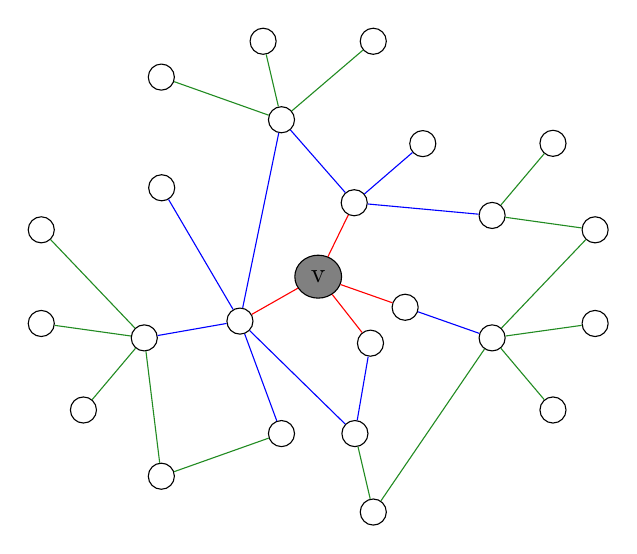
\begin{tikzpicture}[>=latex,line join=bevel,]
%%
\node (b4) at (58.264bp,80.697bp) [draw,ellipse] {};
  \node (b5) at (107.65bp,46.247bp) [draw,ellipse] {};
  \node (b6) at (134.09bp,46.247bp) [draw,ellipse] {};
  \node (b7) at (183.48bp,80.697bp) [draw,ellipse] {};
  \node (b0) at (183.48bp,124.78bp) [draw,ellipse] {};
  \node (b1) at (158.52bp,150.63bp) [draw,ellipse] {};
  \node (b2) at (107.65bp,159.23bp) [draw,ellipse] {};
  \node (b3) at (64.526bp,134.74bp) [draw,ellipse] {};
  \node (c11) at (64.398bp,30.901bp) [draw,ellipse] {};
  \node (c10) at (36.354bp,54.739bp) [draw,ellipse] {};
  \node (a1) at (92.698bp,86.739bp) [draw,ellipse] {};
  \node (a0) at (133.84bp,129.35bp) [draw,ellipse] {};
  \node (c9) at (21.176bp,85.884bp) [draw,ellipse] {};
  \node (a2) at (139.69bp,78.794bp) [draw,ellipse] {};
  \node (c3) at (140.7bp,18.0bp) [draw,ellipse] {};
  \node (c2) at (220.56bp,85.884bp) [draw,ellipse] {};
  \node (c1) at (205.39bp,54.739bp) [draw,ellipse] {};
  \node (c0) at (220.56bp,119.6bp) [draw,ellipse] {};
  \node (c7) at (205.39bp,150.74bp) [draw,ellipse] {};
  \node (c6) at (64.398bp,174.58bp) [draw,ellipse] {};
  \node (c5) at (101.04bp,187.48bp) [draw,ellipse] {};
  \node (c4) at (140.7bp,187.48bp) [draw,ellipse] {};
  \node (a3) at (152.17bp,91.719bp) [draw,ellipse] {};
  \node (c8) at (21.176bp,119.6bp) [draw,ellipse] {};
  \node (v) at (120.87bp,102.74bp) [draw,fill=gray,ellipse] {v};
  \draw [red,] (v) ..controls (135.03bp,84.728bp) and (135.11bp,84.621bp)  .. (a2);
  \draw [ForestGreen,] (b6) ..controls (138.26bp,28.429bp) and (138.28bp,28.341bp)  .. (c3);
  \draw [blue,] (a1) ..controls (80.328bp,107.82bp) and (76.815bp,113.8bp)  .. (b3);
  \draw [ForestGreen,] (b7) ..controls (166.4bp,55.662bp) and (157.67bp,42.867bp)  .. (c3);
  \draw [blue,] (a0) ..controls (121.21bp,143.76bp) and (120.45bp,144.63bp)  .. (b2);
  \draw [ForestGreen,] (b2) ..controls (87.533bp,166.37bp) and (84.387bp,167.49bp)  .. (c6);
  \draw [ForestGreen,] (b4) ..controls (41.841bp,97.922bp) and (37.585bp,102.39bp)  .. (c8);
  \draw [red,] (v) ..controls (142.36bp,95.175bp) and (142.44bp,95.145bp)  .. (a3);
  \draw [ForestGreen,] (b7) ..controls (199.9bp,97.922bp) and (204.16bp,102.39bp)  .. (c0);
  \draw [blue,] (a0) ..controls (147.71bp,141.31bp) and (147.8bp,141.39bp)  .. (b1);
  \draw [ForestGreen,] (b0) ..controls (195.28bp,138.77bp) and (195.36bp,138.87bp)  .. (c7);
  \draw [ForestGreen,] (b4) ..controls (61.028bp,58.262bp) and (61.616bp,53.483bp)  .. (c11);
  \draw [ForestGreen,] (b2) ..controls (103.48bp,177.05bp) and (103.46bp,177.14bp)  .. (c5);
  \draw [blue,] (a1) ..controls (74.544bp,83.554bp) and (74.414bp,83.531bp)  .. (b4);
  \draw [red,] (v) ..controls (130.88bp,123.29bp) and (130.94bp,123.4bp)  .. (a0);
  \draw [ForestGreen,] (b7) ..controls (195.28bp,66.71bp) and (195.36bp,66.613bp)  .. (c1);
  \draw [blue,] (a0) ..controls (156.36bp,127.28bp) and (160.96bp,126.85bp)  .. (b0);
  \draw [ForestGreen,] (b4) ..controls (46.458bp,66.71bp) and (46.377bp,66.613bp)  .. (c10);
  \draw [blue,] (a3) ..controls (169.4bp,85.652bp) and (169.52bp,85.612bp)  .. (b7);
  \draw [ForestGreen,] (b5) ..controls (87.533bp,39.109bp) and (84.387bp,37.993bp)  .. (c11);
  \draw [ForestGreen,] (b2) ..controls (123.17bp,172.5bp) and (124.91bp,173.98bp)  .. (c4);
  \draw [blue,] (a1) ..controls (99.753bp,67.634bp) and (100.57bp,65.415bp)  .. (b5);
  \draw [blue,] (a2) ..controls (136.61bp,60.878bp) and (136.59bp,60.759bp)  .. (b6);
  \draw [red,] (v) ..controls (100.85bp,91.371bp) and (100.71bp,91.289bp)  .. (a1);
  \draw [blue,] (a1) ..controls (110.72bp,69.108bp) and (116.32bp,63.636bp)  .. (b6);
  \draw [blue,] (a1) ..controls (98.712bp,115.9bp) and (101.69bp,130.32bp)  .. (b2);
  \draw [ForestGreen,] (b7) ..controls (201.88bp,83.271bp) and (202.17bp,83.312bp)  .. (c2);
  \draw [ForestGreen,] (b4) ..controls (39.861bp,83.271bp) and (39.566bp,83.312bp)  .. (c9);
  \draw [ForestGreen,] (b0) ..controls (201.88bp,122.21bp) and (202.17bp,122.17bp)  .. (c0);
%
\end{tikzpicture}


}
\caption{Example of the edges present in the calculation of the \emph{Higher Order User Data} for a certain node $v$. \textcolor{red}{Red} edges represent edges whose features are accumulated in the \emph{User Data of Order 0}, \textcolor{blue}{blue} edges represent those of \emph{Order 1}, and \textcolor{ForestGreen}{green} those of \emph{Order 2}.}
\label{fig:higherorderuserdata}
\end{figure}

\subsection{Categorical User Data --- Level $\cat_n$}
\label{subsec:categoricaluserdata}

Another approach to building features for the test is to combine the information contained in $E$, the list of edges, with the one in the ground truth $T \subseteq V$, which says whether a certain node represents a person of \emph{High Income} or a person of \emph{Low Income}.

A simple way to do that is to do an approach similar to the \emph{User Data} presented in \cref{subsec:user_data}, but further discriminating each feature which corresponds to a node $v \in V$ and an edge $e \in E$ when $t \in T$ is the other endpoint of $e$ on whether $t$ corresponds to a person with high or low income. The resulting new features are of the form represented by the set in \cref{eq:matcatuserdata}.

\begin{equation}
\begin{Bmatrix} in \\ out \end{Bmatrix}
\times
\begin{Bmatrix} calls \\ time \\ sms \\ contacts \end{Bmatrix}
\times
\begin{Bmatrix} low \\ high \end{Bmatrix}
\label{eq:matcatuserdata}
\end{equation}

It's important to keep in mind that not all edges of $G$ will be accumulated to these features. Indeed, the majority of users in the testing set $T$ don't have any neighbour that's also in $T$, and thus every feature in this category ends up being $0$.

For completeness sake the set of nodes $F \subseteq T$ is defined as the nodes in the \emph{Inner Graph} (in contrast to the \emph{Outer Graph}, that contains all nodes in $T$), where $F$ only contains nodes which have at least one neighbour with socioeconomic information. In \cref{sec:results} we'll include information about both graphs, and naturally the results on the \emph{Inner Graph} will be better than the ones in the \emph{Outer Graph}, since it contains more information.

Creating these features naïvely will occur in overfitting, since the features are generated by data that's also used for training the supervised learning models. To solve this, the set $T$ is partitioned into two disjoint sets, $G$ and $H$, where $G$ contains roughly 0.75 of the nodes in $T$ is used to calculate the features, while $H$ contains the other 0.25 and is used to train the models.

It's possible to use the method presented in \cref{subsec:higherorderuserdata} generate an \emph{Ego Network of level $n$} of a certain node $v$, and accumulate the adjacent nodes to that network by socioeconomic level before accumulating their data. We refer to the level of these features as $\cat_n$.


\section{The Bayesian Method}
\label{inference_methodology}

%For the SEI:

%Census data + geolocalization + ARPU + cellphone payments (recharges) --> SEI estimation for geolocalized users.

%Second, we extended our predictions taking advantage of graph structure and socioeconomic homophily. To this end, we considered a bayesian

%\sout{As part of the dataset from the bank \( B \), we have the monthly salaries of most bank users \( B_{S_0} \cdots B_{S_t} \) for a period \( t \) larger than \( M \). We considered the average of \( B_{S_i} \) for a period of \( 6 \) moths to generate \( B_S \)}

%\sout{To infer the monthly salary of the users we take the average of \( B_{S_i} \) for a period of \( 6 \) moths to generate \( B_S \), and we compare them with other users' salaries by using the link correlations in \( G_N \).}

\subsection{Income Homophily}

\begin{figure}[h]
\begin{center}
{\includegraphics[width=\columnwidth] % ,trim={0.7cm 1.1cm 2.5cm 1.4cm},clip=true]
{figures/Homophily_income_origin_target_1/Homophily_income_origin_target_1.png}}
\caption{Heatmap showing the number of calls between users, according to their monthly income. There is a higher probability that the callee and the caller have similar income levels.}
\label{homophily_heatmap}
\end{center}
\end{figure}

The main contribution of this work is the estimation of the income of the telco users for which we lack banking data, but have bank clients in their neighborhood of the network graph. To show the feasibility of this task, we first show the existence of a strong income homophily in the telco graph as is evidenced in \Cref{homophily_heatmap}.

For each pair \( \left< o, d \right> \in \mathlarger{G} \), we define \( X \) as the set of incomes for callers and \( Y \) as the set of incomes for callees. According to what we can observe in \Cref{homophily_heatmap}, \( X \) and \( Y \) should be significantly correlated. Given the broad non-Gaussian distribution of the income's values, we choose to use a rank-based measure of correlation which is robust to outliers.

Namely we computed the \textit{Spearman's rank correlation} defined in \cref{spearman} to test the statistical dependence of sets \( X \) and \( Y \). This coefficient gives us a correlation coefficient of \( \mathbf{r_s = 0.474} \). We also compared our result with a randomized null hypothesis, where links between users are selected randomly disregarding income data, obtaining a \( p \)-value of \( p < 10^{-6} \). These values for \( r_s \) and \( p \) show a strong indication of income homophily among users in our communication graph. This observation is consistent with the results reported in~\cite{leo2015socioeconomic}.

We can take advantage of this homophily to propagate income information to the rest of our graph \( \mathP \), where we don't know the income of all the users.

\subsection{Prediction Algorithm}

Instead of predicting the exact value of a user's income, our strategy is to distinguish between only two income categories, \( R_1 = \closeopen{1000}{6300} \) and \( R_2 = \closeopen{6300}{\infty} \), that is, users with low or high income respectively, which we place into two distinct groups \( H_1, H_2 \subseteq G \) depending on \( g_s \), the users' income:
\[
	g \in H_i \iff g_s \in R_i
\]

We define the set \( Q \) as the group of users having at least one connection link to bank clients. For each user \( q^j \in Q \), we compute the number of outgoing calls \( a^j_i \) to the category \( H_i \). Our hypothesis, given the observed homophily, is that if a user \( q^j \) has a higher number of calls \( a^j_i \) to the category \( H_i \) than the other category, it would be more likely to belong to the \( H_i \) income category. In other words, a person is usually in the same income category as the majority of people it calls.

A straightforward approach would be to define the income category of a user as the category where most of its contacts belong. The problem with this approach is that it does not factor in the higher uncertainty in our estimates for users with fewer calls. To address this uncertainty, instead of using calling frequencies to define the probability of a user belonging to the high income category, we use the amount of calls \( a^j_i \) as parameters defining a Beta distribution for the probability of belonging to a given category. We have therefore taken a Bayesian rather than a frequentist approach to income prediction.

We define \(\Beta^j\) as the Beta probability distribution function for each user, which defines a distinct distribution for each user. Having obtained the Beta distribution for the probability of belonging to the high income category, we then find the lowest 5\textsuperscript{th} percentile \( p_{\operatorname{lower}} \) for this probability. If \( p_{\operatorname{lower}} \) is above a given threshold \( \tau \), we set the user's income to \( H_2 \), otherwise we set his income category to \( H_1 \). We note that this criteria takes into account both the mean and the broadness (uncertainty) of the distribution. We also note that the category assigned to a user depends not only on its Beta distribution but also on our choice of \( \tau \).

%We therefore choose a value for \( \tau \) which maximizes the trade off between true positive (\( TPR \)) and false positive (\( FPR \)) rates: \( TPR=TP/P \) and \( FPR=FP/N \) where \( TP \) is the number of correctly predicted users with high income, \( P \) is the total number of users with high income, \( FP \) is the number of users incorrectly classified as having high income, and \( N \) is the total number of users with low income.

%For each user \( q^j \) we estimate and the corresIn this way we obtained a Dirichlet distribution for each user \( q^j \) and compute

%According to the Dirichlet Distibution, each user has a caller income category probability density function of the form

%For all the other users in the telco having at least one link to any other telco user with a defined income \( q \in Q = \left\{x \in \left( N \setminus B \right) \mid (\exists y \in G) \left< x, y \right> \in P \vee \left< y, x \right> \in P \right\} \), we can use this distribution to infer the probabilities of being part of each group \( H_1, \ldots, H_5 \), and this way approximate the economic status.


\section{Results}

% \subsection{Validation Process}

%We need to make sure that our inference algorithm correctly predicts users' income in each of the 5 categories $ H_1, \ldots, H_5 $. According to our hypothesis, the greater the amount of calls to , this increases the probability that both of them will belong to the same group.

%For each link $ p = \left< p_o, p_d, \ldots \right> \in P $, our hypothesis says that $ p_o $ and $ p_d $ will belong to the same income group. 

%In order to validate our proposed methodology, we take advantage of the computed $p_lower$ for each user and use this quantity as the predicition score that allow us to evaluate whether a given user belongs to one of the deffined categories. A standarized way to quantify the performace of the metodology is by computing Receiver Operating Characteristic Curve (ROC). This curve  

We describe in this section the validation of our methodology. 
We examine the true positive ($TPR$) and false positive ($FPR$) rates: 
$$TPR=TP/P \; \; \mbox{ and } \; \;  FPR=FP/N$$ 
where $TP$ is the number of correctly predicted users with high income, $P$ is the total number of users with high income, $FP$ is the number of users incorrectly classified as having high income, and $N$ is the total number of users with low income. 

In Figure~\ref{ROC_multiclass} we plot the ROC (\textit{Receiver Operating Characteristic}) curve, showing $TPR$ and $FPR$ for the set of possible values of $\tau$. We see that our methodology clearly outperforms random guessing (dashed straight line). We can summarize our performance by calculating  the AUC (\textit{Area Under the Curve}) which in Figure~\ref{ROC_multiclass} is $AUC = 0.74$. Note that random guessing would give a value of $AUC \simeq 0.50$.


%\vspace{1em}
%
%\begin{adjustwidth}{-1.5cm}{}
%\begin{tabu} to \textwidth { r X[c] X[c] }
%& \multicolumn{2}{ c }{\textbf{Classifier result for income group $ H_i $}} \\
%\\
%& Caller in group & Caller not in group \\
%Callee in group & \cellcolor{green} True Positive & \cellcolor{red} \makecell{False Negative \\ (Type II Error)} \\ 
%Callee not in group & \cellcolor{red} \makecell{False Positive \\ (Type I Error)} & \cellcolor{green} True Negative \\
%\end{tabu}
%\end{adjustwidth}

%To validate these classifiers, we use 

%a \textbf{Receiver Operating Characteristic Curve} (ROC) to plot the \textbf{True Positive Rate} and the \textbf{False Positive Rate} of each system. Since the amount of people in each group is almost equal, randonly guessing each user's income would result in a diagonal line.

%As an objective measurement, we can calculate the \textbf{Area under the curve} for each income group as the chance that the classifier would make a better prediction of the composition of this income group better than a random one. For this we define the density functions $ f_i(x) $ as the probability that a user will be considered part of the income group $ H_i $, and $ g_i(x) $ as the probability that it won't. This way we can characterize the True Positive Rate and the False Positive Rate for each group as

%\vspace{-1em}
%
%\begin{align*}
%\operatorname{TPR}_i(T) &= \int^{\infty}_T f_i(x) dx \\
%\operatorname{FPR}_i(T) &= \int^{\infty}_T g_i(x) dx \\
%\end{align*}
%
%\vspace{-1.5em}

%With this two functions, we can define the AUC for each category as as a simple integration:

%\[
%A_i = P(X_1 > X_0) = \int^{-\infty}_{\infty} \operatorname{TPR_i}(T) \operatorname{FPR_i}(T) dT
%\]

%Where $ X_1 $ is the score for a positive instance, and $ X_0 $ is the score for a negative one.

%\subsection{Results}

\begin{figure}[H]
\begin{center}
\includegraphics[width=\columnwidth]{figures/ROC_BETA/ROC_Beta_based_approach_201504.png}
\caption{ROC curve for prediction procedure. We observed an $AUC = 0.74$ indicating that our predictor is better than a random predictor ($AUC \simeq 0.50$).}
\label{ROC_multiclass}
\end{center}
\end{figure}

%The result ROC curves have the following areas:
%
%\vspace{-1em}
%
%\begin{align*}
%A_1 &= 0.68 & A_2 &= 0.69 & A_3 &= 0.63 \\ 
%A_4 &= 0.68 & A_5 &= 0.69
%\end{align*}
%
%As evidenced by figure \ref{ROC_multiclass}, the inference process seems to have been successful: the predicted value is much better than one predicted by a random classifier for all of the categories.


\bibliography{../Tesis/bibliography/sna}{}

\end{document}
